\documentclass[12pt]{article}
\usepackage[a4paper, margin=.30in]{geometry}
\usepackage{graphicx ,
            wrapfig,
            xcolor, 
            enumerate,
            amsmath,fontenc, mhchem
            }

\newcommand\headerMe[2]{\noindent{}#1\hfill#2}
\renewcommand{\thesection}{\Roman{section}}

\author{Zakaria HAOUZAN}
\date{\today}

\begin{document}
% headers --------------
\headerMe{Matière : Physique-Chimie}{Professeur : Zakaria HAOUZAN}\\
\headerMe{Unité : Transformations lentes et rapides\\ d'un système chimique }{Établissement : Lycée SKHOR qualifiant}\\
\headerMe{Niveau : 2BAC-SM-X}{Heure : 11H}\\

% ------Content ________
\begin{center}

    \Large{Leçon $N^{\circ} 2.2 $: \color{red} Suivi temporel d’une transformation - Vitesse de réaction }
\end{center}

%\begin{figure}[h!]
	%\begin{center}
	%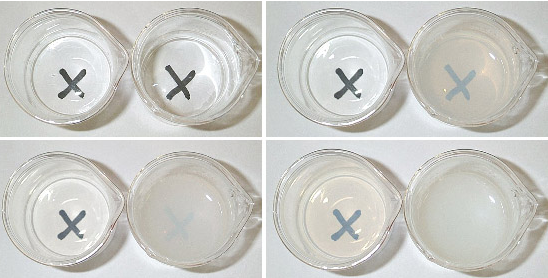
\includegraphics[width=0.5\textwidth]{./img/TRLconcentration.png}
%\end{center}
%\vspace{-1cm}
%\end{figure}



%\begin{wrapfigure}[10]{r}{0.5\textwidth}
%    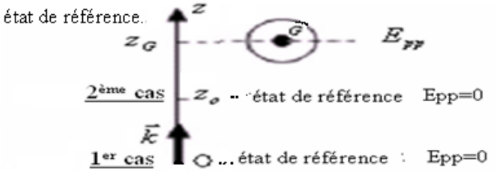
\includegraphics[width=0.5\textwidth]{./img/img00.png}
%\end{wrapfigure}


%\begin{center}
   %\begin{tabular}{|c|c|c|}
      %\hline
      %Indicateur coloré & Couleur de l’espèce acide & Couleur de l’espèce base\\\hline
      %BBT               & Jaune                     & Bleue\\\hline
      %Hélianthine       &Rose                       & Jaune\\\hline
      %Phénolphtaléine   & inclore                   & rose \\\hline
   %\end{tabular}
%\end{center}

\section{Techniques de suivi temporel d'une transformation :}

Pour suivre temporellement l'évolution d'une transformation chimique on doit connaître sa composition à chaque instant.
Il existe plusieurs méthodes qui permettent de suivre l'évolution d'une transformation chimique : 
\\- Le dosage.
- La conductimétrie.
- La mesure de la pression.
- La pH-métrie.

\begin{wrapfigure}[1]{r}{0.3\textwidth}
	\vspace{-3cm}
	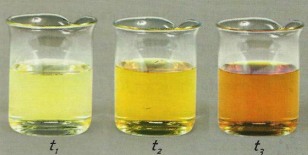
\includegraphics[width=0.27\textwidth]{./img/STidureavecperoxo.png}
\end{wrapfigure}



\section{suivi temporel d'une transformation :  }
\subsection{Le Dosage : }
\subsubsection{Expérience : }
Dans un bécher, verser 50 mL d'une solution incolore de peroxodisulfate de potassium, 
$(2K^+_{(aq)} + {S_2O_8^{2-}}_{(aq)})$, à $0,10 mol.L^{-1}$ puis 50 mL d'une solution, incolore elle aussi, d'iodure de potassium, $(K^+_{(aq)} +I^-_{(aq)})$.
à $0.50 mol.L^-$


\subsubsection{Exploitation :}
\begin{itemize}
	\item L'apparition progressive de la coloration jaune, caractéristique des molécules ${I_2}_{(aq)}$, montre que ces molécules sont formées par une réaction lente entre les ions peroxodisulfate ${S_2O_8}^{2-}$ et les ions iodure$I^-$. 

\item Les ions peroxodisulfate $S_2O_8^{2-}$ oxydent les ions iodure $I^-$ selon une réaction d'équation: 

	$2I^-_{(ag)} + {S_2O_8^{2-}}_{(aq)} = {I_2}_{(aq)} + 2{SO_4^{2-}}_{(aq)}$ (1)

	\item Cete réaction nétant pas trop rapide, elle peut être suivie en dosant le
diode formé.

\item On peut également utiliser la spectrophotométrie puisque la réaction met en jeu une seule espèce colorée, le diiode.

\item Les ions iodures $I^-$ sont lentement oxydés par les ions peroxodisulfate ce qui entraine la formation progressive du diiode $I_2$.
Pour savoir la quantité du diiode qui s'est formée à un instant donné on réalise le dosage de la manière suivante:

\item On recueille après chaque trois minutes $10cm^3$ du mélange réactionnel et on la trempe dans l'eau froide pour arrêter la réaction,Puis on dose le diiode $I_2$ formé par une solution de thiosulfate de sodium $(2Na^+ + {S_2O_3}^{2-})$  de concentration $Cr= 0,02mol/L$.


%\begin{figure}[h!]
	\begin{center}
	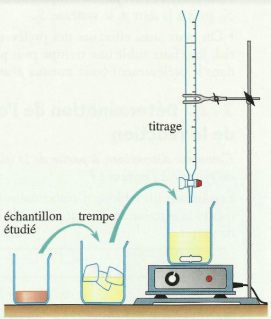
\includegraphics[width=0.3\textwidth]{./img/STlatrempe.png}
	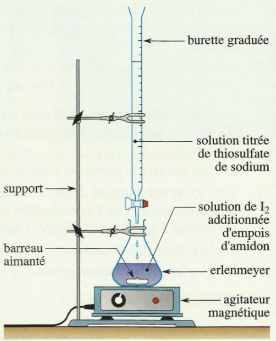
\includegraphics[width=0.3\textwidth]{./img/STmotageDosage.png}
\end{center}

%\end{figure}
\item Les deux couples mis en jeux durant le dosage sont :$I_2/I^-$ ET $S_4O_6^{2-}/S_2O_3^{2-}$.
\item Equation de la réaction du dosage: \ce{2S_2O_3^{2-} + I_2 -> S_4O_6^{2-} + 2I^-}
c'est une réaction rapide 
\item à l'équivalence : $\frac{n(S_2O_3^{2-})}{2} = \frac{n(I_2)}{1}$

\item Soit vr le volume de la solution de thiosulfate de sodium ajoutée à l'équivalence. $n(I_2) = \frac{C_r.V_r}{2}$

\item Tableau des mesures: 

\begin{center}
   \begin{tabular}{|c|c|c|c|c|c|c|c|c|c|c|c|}
	  \hline
	  t(s)         &0&3  &6&9&12&16&20&30&40&50&60 \\\hline
	  n($I_2 mmol$)&0&0.5&1.0 &1.4&1.7&2.1&2.3&2.8&3.1&3.2&3.3\\\hline
   \end{tabular}
\end{center}

\item Tableau d'avancement

\begin{tabular}{|c|c|c|c|c|c|}
    \hline
	\multicolumn{2}{|c|}{Equation de la réaction}& \multicolumn{4}{c|}{${ S_2O_8^{2-} + 2I^- \rightarrow 2S_2O_4^{2-} + I_2}$}\\\hline
    états  & avancement& \multicolumn{4}{|c|}{quantité de Matière en mol}\\\hline
    Etat initial          &    0        & $ C_2.V_2$   & $ C_1.V_1$  & $ 0$     & $ 0$ \\\hline
    Etat de transformation&    $x$      & $ C_2.V_2 - x$ & $ C_1.V_1 -  2x$      & $ 2x$        & $ x$ \\\hline
    Etat final            &    $x_{max}$& $  C_2.V_2 - x_{max}$ & $  C_1.V_1 - 2x_{max}$& $2x_{max}$  & $  x_{max}$ \\\hline
   % \cline{2-4}\
\end{tabular}

\item D'après le tableau d'avancement, la quantité du diiode formée à un instant t est égale à x.${n(I_2)}_t$=$x$. Donc le dosage nous permet de suivre l'évolution de la formation du diiode en fonction du temps et de déterminer l'avancement.

	\begin{center}
	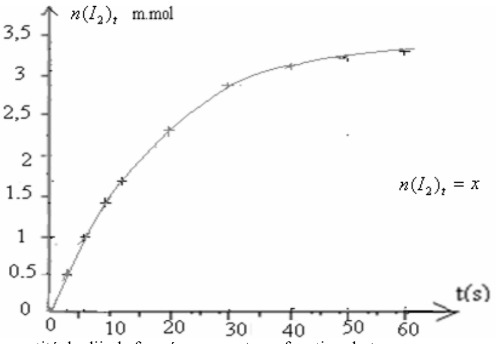
\includegraphics[width=0.3\textwidth]{./img/STcourbeI2.png}
	\hspace{1cm}
	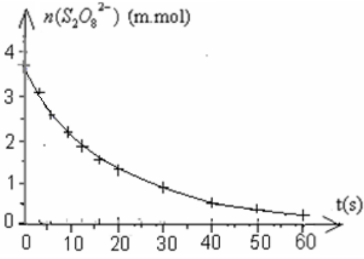
\includegraphics[width=0.3\textwidth]{./img/STcourbeS_2.png}
\end{center}



\item Le tracé montre que la quantité du diiode formée augmente en fonction du temps.
On peut déterminer les quantités de matières des autres constituants du mélange réactionnel en fonction du temps. 

\item Exemple : $n(S_2O_8^{2-}) = C_2.V_2 - x$ avec $C_2 = 0.036mol/L$  et $V_2 = 100ml$ donc $n(S_2O_8^{2-}) = 3.6 - x $

\begin{center}
   \begin{tabular}{|c|c|c|c|c|c|c|c|c|c|c|c|}
	  \hline
	  t(s)         &0&3  &6&9&12&16&20&30&40&50&60 \\\hline
	  $x (mmol$)   &0&0.5&1.0 &1.4&1.7&2.1&2.3&2.8&3.1&3.2&3.3\\\hline
	  n($S_2O_8^{2-} mmol$)&3.6&3.1&2.6 &2.2&1.9&1.5&1.3&0.8&0.5&0.4&0.3\\\hline
   \end{tabular}
\end{center}

Le tracé décroissant montre que la quantité de $S_2O_8^{2-}$ diminue en fonction du temps.

\end{itemize}

\begin{wrapfigure}[2]{r}{0.3\textwidth}
	\vspace{-3cm}
	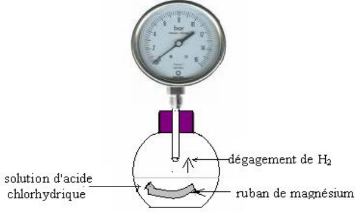
\includegraphics[width=0.3\textwidth]{./img/STpressionavec_balon.png}
\end{wrapfigure}


\section{Méthode de mesure de la pression : }
\subsection{Expérience: }
On introduit un ruban de magnésium de masse $m=0,02g$ dans ballon contenant un volume $V=50cm3$
d'une solution d'acide chlorhydrique ($H^+_{(aq)} + Cl^-_{(aq)}$) de concentration $C=0,5mol/L$ puis on mesure la pression du gaz résultant par un manomètre.

\vspace{0.2cm}

On constate que le magnésium réagit avec l'acide chlorhydrique avec dégagement d'hydrogène et cette réaction dure quelques
minutes jusqu'à la disparition totale du ruban de magnésium.
Ecrire l'équation de la réaction sachant que les deux couples mis en jeux sont : $H^+/H_2$ et $Mg^{2+}/Mg$

\ce{$Mg_{(s)} + 2H^+$ -> $Mg^{2+}_{(aq)} + {H_2}_{(g)}$}

%\begin{wrapfigure}[2]{r}{0.2\textwidth}
%\end{wrapfigure}


\subsection{Exploitation:}
\begin{itemize}
	\item La quantité de matière initiale du magnésium : $n_0(Mg) = \frac{m(Mg)}{M(Mg)} = \frac{0.02g}{24.3g/mol} = 0.82mmol$
	\item La quantité de matière initiale des ions $H^+$: ${n_0(H^+)}_{(aq)} = c.v = 0.5mol/L . 50.10^{-3}mol = 25mmol$
\item Tableau d'avancement

\begin{tabular}{|c|c|c|c|c|c|}
    \hline
	\multicolumn{2}{|c|}{Equation de la réaction}& \multicolumn{4}{c|}{$ Mg + 2H^+ \rightarrow  Mg^{2+} + H_2$}\\\hline
    états  & avancement& \multicolumn{4}{|c|}{quantité de Matière en mol}\\\hline
    Etat initial          &    0    & $ 0.82$   & $ 25$  & $ 0$     & $ 0$ \\\hline
    Etat de transformation&    $x$  & $ 0.82- x$ & $ 25-2x$ & $ x$        & $ x$ \\\hline
    Etat final            &    $x_{max}$& $ 0.82-x_{max}$ & $25- 2x_{max}$& $x_{max}$  & $  x_{max}$ \\\hline
   % \cline{2-4}\
\end{tabular}

\item Or la réaction continue jusqu'à la disparition totale du ruban de magnésium, Mg est le réactif limitant. $x_{max} = 0.82mmol$ 
\item D'après le tableau d'avancement à un instant t(état de transformation) $n(H_2)$ et à état final $n(H_2)$=$x_{max}$

\item la pression est liée à la quantité de matière du l'hydrogène gazeux résultant de la réaction par la relation $${P}_{(H_2)}.V = n_{(H_2)}.R.T \hspace{1cm} P_{(H_2)} =\frac{n_{(H_2)}.R.T}{V} \hspace{2cm}  (1)$$

\item À l'instant t=o la pression dans le ballon est égale à la pression atmosphérique. 
\item À un instant t la pression dans le ballon (indiquée par le manomètre) est : $P = P_{atm} + P_{(H_2)}$ donc $P_{(H_2)}= P-P_{atm}$

\item Donc à un instant t la relation (1) devient : $ P_{(H_2)}= P_t-P_{atm} = \frac{x.R.T}{V}$ (1')

\item Et à la fin de la réaction elle devient : $ P_{(H_2)}= P_{max}-P_{atm} = \frac{x_{x_{max}}.R.T}{V}$ (1")

	En divisant (1') par (1") on obtient ($x = n(H_2)$): $$x = \frac{P_t-P_{atm}}{P_{x_{max}}-P_{atm}}$$ 

\begin{center}
	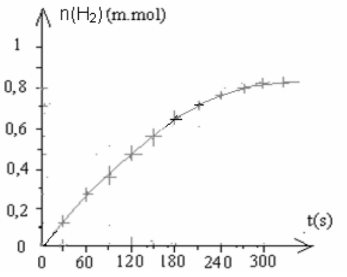
\includegraphics[width=0.2\textwidth]{./img/STcourbepressionH_2.png}
\end{center}

	
\item Tableau des mesures:($P_{atm}=1013hPa$ et $P_{max}=1093hPa$) 

\begin{center}
   \begin{tabular}{|c|c|c|c|c|c|c|c|c|c|c|c|c|}
	  \hline
	  t(s)       &0     &30  &60  &90  &120 &150 &180 &210 &240 &270 &300&330 \\\hline
	  P($hPa$)   &1013  &1025&1036&1048&1060&1068&1097&1081&1087&1091&1093&1093\\\hline
	  x($mmol$)  &0     &0.12&0.24&0.36&0.48&0.56&0.68&0.7&0.76 &0.8 &0.82& 0.82\\\hline
   \end{tabular}
\end{center}
\end{itemize}

\section{Méthode de mesure de la conductance : }
\subsection{Expérience : }
On introduit dans un bécher un peu d'eau et d'éthanol et on ajoute au mélange $1cm^3$ de 2-chloro 2-méthyle propane de formule semi-développée : $(CH_3)-C-Cl$ qu’on notera simplement $R-Cl$.

L'éthanol est un solvant dans lequel RCL se dissout très facilement et sans réagir avec l'éthanol.$RCl$ réagit avec l'eau selon
l'équation suivante: \ce{R-Cl + H_2O -> H^+ + Cl^-}

La formation des ions $H^+$ et $Cl^-$ entraine l'augmentation de la conductance de la solution.

On mesure la conductance du mélange réactionnel chaque $200s$ ce permet de déterminer la variation de sa conductivité en fonction du temps.

\begin{center}
   \begin{tabular}{|c|c|c|c|c|c|c|c|c|c|c|c|}
	  \hline
	  t(s)         &0&200  &400   &600  & 800 &1000 &1200 &1400 &1600 &1800 &2000 \\\hline
	  $\sigma(S/m)$&0&0.489&0.977 &1.270&1.466&1.661&1.759&1.856&1.905&1.955&1.955\\\hline
   \end{tabular}
\end{center}
\subsection{Exploitation: }
\begin{itemize}
\item la quantité de matière initiale avec $\rho(R-Cl) = 0.85g/cm^3$ et $M(R-Cl) = 92.5 g/mol$  

	$n_0 = \frac{m}{M} =\frac{\rho.V}{M} = \frac{0.85g/cm^3 . 1cm^3}{92.5 g/mol} \approx 9.2 10^{-3} mol$
\item Tableau d'avancement

\begin{tabular}{|c|c|c|c|c|c|c|}
    \hline
	\multicolumn{2}{|c|}{Equation de la réaction}& \multicolumn{5}{c|}{$ R-Cl + H_2O \rightarrow  R-OH + H^++ Cl^-$}\\\hline
    états  & avancement& \multicolumn{5}{|c|}{quantité de Matière en mol}\\\hline
	Etat initial          &    0    & $ n_0$   & par excès  & $ 0$     & $ 0$ &0 \\\hline
	Etat de transformation&    $x$  & $ n_0- x$ & par excès& $ x$        & $ x$&x \\\hline
	Etat final            &$x_{max}$& $ n_0-x_{max}$ & par excès& $x_{max}$  & $  x_{max}$& $  x_{max}$\\\hline
   % \cline{2-4}\
\end{tabular}

H2O étant utilisée en excès , RCl est le réactif limitant . $x_{max} = n_0$

\item La conductivité de la solution est : $$\sigma = \lambda_{H^+}.[H^+] + \lambda_{Cl^-}.[Cl^-]$$

	On a : $\sigma = (\lambda_{H^+} + \lambda_{Cl^-}).\frac{x}{V}$ et $[H^+]= [Cl^-] =\frac{x}{V}$ 
	Donc : $$\sigma_t = (\lambda_{H^+} + \lambda_{Cl^-}).\frac{x}{V} \hspace{1cm} (1) $$
$$\sigma_{max} = (\lambda_{H^+} + \lambda_{Cl^-}).\frac{x_{max}}{V} \hspace{1cm}  (2)$$

\item En divisant (1) par (2) on obtient: $x = \frac{\sigma_t}{\sigma_{max}}. x_{max}$

\item Tableau des mesures:($\sigma_{max}=1.955Sm^{-1}$ et $x=\frac{\sigma_t.9.210^{-3}}{1.955}$) 

\begin{center}
   \begin{tabular}{|c|c|c|c|c|c|c|c|c|c|c|c|c|}
	  \hline
	  t(s)         &0&200  &400  &600  &800  &1000 &1200 &1400 &1600 &1800 &2000&2200 \\\hline
	  $\sigma(S/m)$&0&0.489&0.977&1.270&1.466&1.661&1.759&1.856&1.905&1.955&1.955&1.955\\\hline
	  x($mmol$)    &0&2.3  &4.6  &5.98 &6.9  &7.82 &8.32 &8.64 &8.96 &9.20 &9.20& 9.20\\\hline
   \end{tabular}
\end{center}
\end{itemize}

\section{Vitesse de la réaction - Temps demi réaction :  }
\subsection{Vitesse de la réaction}
\section*{Définition:}
La vitesse volumique d’une réaction correspond à la quantité de matière formée ou disparue par unité de temps et de volume.
Elle est liée à la variation de l’avancement x de la réaction en fonction du temps par la relation suivante:
$$v = \frac{1}{V}.\frac{dx}{dt}$$

$v : $ vitesse volumique de la réaction en ($mol/m^3.s$).

$\frac{dx}{dt}$ : dérivée de l'avancement en (mol/s)

$V$ : volume totale de la solution.

En général, la vitesse de la réaction diminue lors de l'évolution d'une transformation chimique. 
\end{document}

